

\documentclass{beamer}
\usepackage[utf8]{inputenc}

\usetheme{Madrid}
\usecolortheme{default}
\usepackage{amsmath,amssymb,amsfonts,amsthm}
\usepackage{mathtools}
\usepackage{txfonts}
\usepackage{tkz-euclide}
\usepackage{listings}
\usepackage{adjustbox}
\usepackage{array}
\usepackage{tabularx}
\usepackage{gvv}
\usepackage{lmodern}
\usepackage{circuitikz}
\usepackage{tikz}
\usepackage{graphicx}
\setbeamertemplate{page number in head/foot}[totalframenumber]
\usepackage[T1]{fontenc}
\usepackage{tcolorbox}
\tcbuselibrary{minted,breakable,xparse,skins}

\definecolor{bg}{gray}{0.95}
\DeclareTCBListing{mintedbox}{O{}m!O{}}{%
  breakable=true,
  listing engine=minted,
  listing only,
  minted language=#2,
  minted style=default,
  minted options={%
    linenos,
    gobble=0,
    breaklines=true,
    breakafter=,,
    fontsize=\small,
    numbersep=8pt,
    #1},
  boxsep=0pt,
  left skip=0pt,
  right skip=0pt,
  left=25pt,
  right=0pt,
  top=3pt,
  bottom=3pt,
  arc=5pt,
  leftrule=0pt,
  rightrule=0pt,
  bottomrule=2pt,
  toprule=2pt,
  colback=bg,
  colframe=orange!70,
  enhanced,
  overlay={%
    \begin{tcbclipinterior}
    \fill[orange!20!white] (frame.south west) rectangle ([xshift=20pt]frame.north west);
    \end{tcbclipinterior}},
  #3,
}

% Code style
\lstset{
    language=C,
    basicstyle=\ttfamily\small,
    keywordstyle=\color{blue},
    stringstyle=\color{orange},
    commentstyle=\color{green!60!black},
    numbers=left,
    numberstyle=\tiny\color{gray},
    breaklines=true,
    showstringspaces=false,
}

% Title info
\title %optional
{Optimization - 2.0.18}
\date{March 26, 2026}
\author % (optional)
{EE25BTECH11018 - Darisy Sreetej}

\begin{document}

\frame{\titlepage}

\begin{frame}{Question}
For the data given below, how many machines can be assigned to an operator to
minimize idle time of the operator and machines $?$
\begin{center}
\begin{tabular}[12pt]{ |c|c|c| } 
    \hline
    Activity & Time (minutes) \\ 
    \hline
    machine loading $+$ unloading & 2\\
    \hline 
    machining & 4 \\
    \hline
     walking from one machine to the next & 1  \\
    \hline   
\end{tabular}
\end{center}

\quad
 \begin{enumerate}

\item   $1$ 
\item   $2$
 \item $3$
\item  $4$

 \end{enumerate}
 \hfill(EC 2007) 
\end{frame}
\begin{frame}{Solution - Identifying Components}
\textbf{Given:}
\begin{enumerate}
  
    \item Service time (loading + unloading): 
    \begin{align}
    S = 2 \text{ min}
    \end{align}
    
    \item Machining time: 
    \begin{align}
    M = 4 \text{ min}
    \end{align}
    
    \item Walking time: 
    \begin{align}
    W = 1 \text{ min}
\end{align}
\end{enumerate}
\end{frame}
\begin{frame}{Solution - Operator Cycle time}
 Consider \textbf{n} machines :

\begin{align*}
\text{Service time} &= nS = 2n \\
\text{Walking time} &= (n-1)W \\
&= (n-1)\cdot 1 \\
&= n-1 \\
\end{align*}
The \textbf{operator cycle time} i.e, the total time taken by the operator to complete one full round of all machines and come back to the starting point
\begin{align*}
 T_o &= nS + (n-1)W \\
&= 2n + (n-1) \\
&= 3n - 1
\end{align*}
\end{frame}


\begin{frame}{Solution - Applying Max-Min conditions}
\textbf{Operator should not be idle:}
\begin{align}
T_o \geq M
\end{align}

\textbf{Substituting:}
\begin{align*}
3n - 1 &\geq 4 \\
3n &\geq 5 \\
n &\geq \frac{5}{3} = 1.67
\end{align*}
Thus , 
\begin{align}
    n &\geq 1.67
\end{align}
\end{frame}


\begin{frame}{Solution - Applying Max-Min conditions}

\textbf{Machine should not wait too long:}

The operator should return before the machine experiences excessive idle time.

\begin{align}
T_o \leq M + S
\end{align}

(The machine runs automatically for time $M$ .After completion, it can tolerate at most one service time delay $S$ .Beyond this, the machine remains idle excessively . So , its $M+S$ )

\begin{align*}
3n - 1 &\leq 4 + 2 \\
3n &\leq 7 \\
n &\leq \frac{7}{3} = 2.33
\end{align*}
Thus , 
\begin{align}
    n &\leq 2.33
\end{align}


\end{frame}




\begin{frame}{Solution - Combining Bounds}

from (5) , (7) :

\begin{align}
   1.67 &\leq n \leq 2.33
\end{align}

Since number of machines must be an integer $ n \in \mathbb{Z} $

Hence, the optimal number of machines assigned to the operator is 2 (option 2)
\end{frame}


\begin{frame}[fragile]
    \frametitle{Python Code}
    \begin{lstlisting}[language=Python]
import cvxpy as cp
import numpy as np
import matplotlib.pyplot as plt

# defining Parameters
t_lu = 2   # loading + unloading
t_m = 4    # machining time
t_w = 1    # walking time

n = cp.Variable(integer=True)

# operator cycle time
T_o = n * t_lu + (n - 1) * t_w   

idle_time_mismatch_expr = cp.abs(T_o - t_m)
objective = cp.Minimize(idle_time_mismatch_expr)

constraints = [n >= 1]
     \end{lstlisting}
\end{frame}


\begin{frame}[fragile]
\frametitle{Python Code}
    \begin{lstlisting}[language=Python]
problem = cp.Problem(objective, constraints)
problem.solve()

optimal_n = int(np.round(n.value))
minimized_idle_time = round(problem.value, 2)

print(f"Optimal Number of Machines (n): {optimal_n}")
print(f"Minimized Idle Time : {minimized_idle_time} minutes")

n_values = np.arange(1, 6)

T_o_values = n_values * t_lu + (n_values - 1) * t_w

idle_time_mismatch = np.abs(T_o_values - t_m)

plt.figure(figsize=(8, 5))
plt.plot(n_values, T_o_values, marker='o', label='Operator Cycle Time (To)')
\end{lstlisting}
\end{frame}


\begin{frame}[fragile]
\frametitle{Python Code}
    \begin{lstlisting}[language=Python]
plt.axhline(y=t_m, linestyle='--', label='Machine Time (M)')
plt.plot(n_values, idle_time_mismatch, marker='s', label='Idle Time Mismatch')

plt.plot(optimal_n, minimized_idle_time, marker='o', markersize=10, label=f'Optimal n={optimal_n}')

plt.xlabel('Number of Machines (n)')
plt.ylabel('Time (min)')
plt.title('Optimal Machine Assignment')
plt.xticks(n_values)
plt.grid(True)
plt.legend()
plt.show()
\end{lstlisting}
\end{frame}

\begin{frame}{Plot}
    \begin{figure}
        \centering
        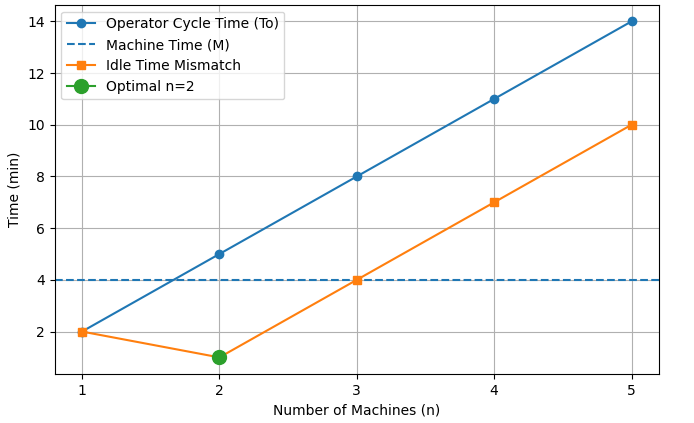
\includegraphics[width=1.0\linewidth]{image.png}
    \end{figure}
\end{frame}
\end{document}





 




